% Practice Test 08 — Alaska Edition
% Questions: 30 (21 MC + 9 SA)
% Generated by scripts/generate_practice_tests.py

\begin{practiceQuestion}{1-3-q13}{mc}
\begin{questionText}
The table shows a proportional relationship. Find the missing value.

\begin{center}
\begin{tabular}{|c|c|}
\hline $x$ & $y$ \\ \hline $4$ & $14$ \\ $6$ & $?$ \\ $10$ & $35$ \\ \hline
\end{tabular}
\end{center}
\end{questionText}
\choiceA{$18$}
\choiceB{$20$}
\choiceC{$21$}
\choiceD{$24$}
\correctAnswer{C}
\explanation{$k = \frac{14}{4} = 3.5$. Missing value: $y = 3.5 \times 6 = 21$. Check: $\frac{35}{10} = 3.5$ \checkmark.}
\end{practiceQuestion}

\begin{practiceQuestion}{1-5-q21}{sa}
\begin{questionText}
A proportional line has slope $\frac{5}{3}$. Find $y$ when $x = 9$ and $x$ when $y = 25$.
\end{questionText}
\correctAnswer{$y = 15$ when $x = 9$; $x = 15$ when $y = 25$}
\explanation{$y = \frac{5}{3} \times 9 = 15$. For $y = 25$: $25 = \frac{5}{3}x$, so $x = 25 \times \frac{3}{5} = 15$.}
\end{practiceQuestion}

\begin{practiceQuestion}{1-6-q26}{gmc}
\begin{questionText}
The table shows the distance a bus travels over several hours. Using proportional reasoning, how far will the bus travel in $9$ hours?

\begin{center}
\begin{tabular}{|c|c|}
\hline
\textbf{Hours} & \textbf{Miles} \\ \hline
$2$ & $90$ \\ \hline
$5$ & $225$ \\ \hline
$7$ & $315$ \\ \hline
$9$ & $?$ \\ \hline
\end{tabular}
\end{center}
\end{questionText}
\choiceA{$360$ miles}
\choiceB{$385$ miles}
\choiceC{$405$ miles}
\choiceD{$450$ miles}
\correctAnswer{C}
\explanation{Rate: $90 \div 2 = 45$ mph. In $9$ hours: $45 \times 9 = 405$ miles.}
\end{practiceQuestion}

\begin{practiceQuestion}{2-2-q10}{mc}
\begin{questionText}
$96$ is $80\%$ of what number?
\end{questionText}
\choiceA{$76.8$}
\choiceB{$100$}
\choiceC{$116$}
\choiceD{$120$}
\correctAnswer{D}
\explanation{$\frac{96}{w} = \frac{80}{100}$. Cross-multiply: $80w = 9600$. Divide: $w = 120$.}
\end{practiceQuestion}

\begin{practiceQuestion}{2-5-q17}{mc}
\begin{questionText}
A freelance artist charges a $\$50$ base fee plus $7\%$ of the project value. For a $\$600$ project, what is the total charge?


\numberLine[100]{0}{700}
\end{questionText}
\choiceA{$\$42$}
\choiceB{$\$92$}
\choiceC{$\$107$}
\choiceD{$\$650$}
\correctAnswer{B}
\explanation{Percent fee: $600 \times 0.07 = \$42$. Total: $50 + 42 = \$92$.}
\end{practiceQuestion}

\begin{practiceQuestion}{3-1-q27}{gmc}
\begin{questionText}
The number line below shows two points. Which statement is correct?

\begin{center}
\begin{tikzpicture}
  \draw[thick,->] (-6.5,0) -- (6.5,0);
  \foreach \x in {-6,...,6} \draw (\x,0.1) -- (\x,-0.1) node[below] {$\x$};
  \fill[funBlue] (-4,0) circle (4pt) node[above=6pt] {P};
  \fill[funBlue] (4,0) circle (4pt) node[above=6pt] {Q};
\end{tikzpicture}
\end{center}
\end{questionText}
\choiceA{P and Q are the same number}
\choiceB{P and Q are opposites}
\choiceC{$|P| > |Q|$}
\choiceD{$P > Q$}
\correctAnswer{B}
\explanation{Point P is at $-4$ and Q is at $4$. They are the same distance from $0$ on opposite sides, so they are opposites.}
\end{practiceQuestion}

\begin{practiceQuestion}{3-2-q04}{mc}
\begin{questionText}
What is $9 + (-14)$?
\end{questionText}
\choiceA{$23$}
\choiceB{$-23$}
\choiceC{$-5$}
\choiceD{$5$}
\correctAnswer{C}
\explanation{Different signs: $14 - 9 = 5$. The larger absolute value ($14$) is negative, so the answer is $-5$.}
\end{practiceQuestion}

\begin{practiceQuestion}{3-3-q12}{mc}
\begin{questionText}
What is $(-3) - 5 - (-10)$?
\end{questionText}
\choiceA{$-18$}
\choiceB{$2$}
\choiceC{$-2$}
\choiceD{$12$}
\correctAnswer{B}
\explanation{Rewrite: $(-3) + (-5) + 10$. Add negatives: $-3 + (-5) = -8$. Then $-8 + 10 = 2$.}
\end{practiceQuestion}

\begin{practiceQuestion}{3-10-q25}{sa}
\begin{questionText}
The lowest point in Lake Baykal is $-5{,}387$ feet. The surface is at $1{,}637$ feet above sea level. How deep is the lake from surface to bottom?
\end{questionText}
\correctAnswer{$7{,}024$ feet}
\explanation{$1{,}637 - (-5{,}387) = 1{,}637 + 5{,}387 = 7{,}024$ feet.}
\end{practiceQuestion}

\begin{practiceQuestion}{4-1-q03}{mc}
\begin{questionText}
Which expression means ``a number $n$ divided by $4$, then increased by $3$''?
\end{questionText}
\choiceA{$\frac{n + 3}{4}$}
\choiceB{$\frac{4}{n} + 3$}
\choiceC{$\frac{n}{4} + 3$}
\choiceD{$4n + 3$}
\correctAnswer{C}
\explanation{``Divided by $4$'' gives $\frac{n}{4}$. ``Increased by $3$'' means add $3$: $\frac{n}{4} + 3$.}
\end{practiceQuestion}

\begin{practiceQuestion}{5-2-q30}{gsa}
\begin{questionText}
The flowchart shows the steps used to get from $x$ to $22$. Work backward to find $x$.

\begin{center}
\begin{tikzpicture}[node distance=2cm, auto, scale=0.8]
  \node[draw,rounded corners,fill=funBlue!15,minimum width=1.5cm] (start) {$x$};
  \node[draw,fill=funOrange!15,minimum width=1.5cm,right of=start] (step1) {$\times 5$};
  \node[draw,fill=funOrange!15,minimum width=1.5cm,right of=step1] (step2) {$- 3$};
  \node[draw,rounded corners,fill=funGreen!15,minimum width=1.5cm,right of=step2] (end) {$22$};
  \draw[->,thick] (start) -- (step1);
  \draw[->,thick] (step1) -- (step2);
  \draw[->,thick] (step2) -- (end);
\end{tikzpicture}
\end{center}
\end{questionText}
\correctAnswer{$x = 5$}
\explanation{The equation is $5x - 3 = 22$. Add $3$: $5x = 25$. Divide by $5$: $x = 5$. Check: $5 \times 5 = 25$, $25 - 3 = 22$ \checkmark.}
\end{practiceQuestion}

\begin{practiceQuestion}{5-3-q19}{sa}
\begin{questionText}
Solve $4(x + 9) = 52$.
\end{questionText}
\correctAnswer{$x = 4$}
\explanation{Divide by $4$: $x + 9 = 13$. Subtract $9$: $x = 4$. Check: $4(4 + 9) = 4(13) = 52$ \checkmark.}
\end{practiceQuestion}

\begin{practiceQuestion}{5-4-q21}{sa}
\begin{questionText}
Solve $\dfrac{x}{2} + \dfrac{x}{4} = 9$.
\end{questionText}
\correctAnswer{$x = 12$}
\explanation{Multiply every term by $4$: $2x + x = 36$. Combine: $3x = 36$. Divide by $3$: $x = 12$. Check: $\frac{12}{2} + \frac{12}{4} = 6 + 3 = 9$ \checkmark.}
\end{practiceQuestion}

\begin{practiceQuestion}{5-5-q07}{mc}
\begin{questionText}
You have $\$60$ and spend $\$8$ per day. You want to have at least $\$12$ left. Which inequality finds the number of days $d$ you can spend?
\end{questionText}
\choiceA{$60 - 8d \leq 12$}
\choiceB{$60 + 8d \geq 12$}
\choiceC{$60 - 8d \geq 12$}
\choiceD{$8d - 60 \geq 12$}
\correctAnswer{C}
\explanation{Start with $\$60$, subtract $\$8$ per day, need at least $\$12$: $60 - 8d \geq 12$.}
\end{practiceQuestion}

\begin{practiceQuestion}{5-6-q02}{mc}
\begin{questionText}
Which graph represents $x \leq -2$?
\end{questionText}
\choiceA{Open circle at $-2$, shade left}
\choiceB{Closed circle at $-2$, shade right}
\choiceC{Closed circle at $-2$, shade left}
\choiceD{Open circle at $-2$, shade right}
\correctAnswer{C}
\explanation{$x \leq -2$: closed circle (includes $-2$) and shade left (values less than or equal to $-2$).}
\end{practiceQuestion}

\begin{practiceQuestion}{6-2-q24}{sa}
\begin{questionText}
A drawing uses $1$ cm $= 7$ m. You redraw at $1$ cm $= 7$ m (the same scale). A line is $5$ cm long. How long is it on the new drawing?
\end{questionText}
\correctAnswer{$5$ cm}
\explanation{The scale ratio is $\frac{7}{7} = 1$. The length stays the same: $5 \times 1 = 5$ cm.}
\end{practiceQuestion}

\begin{practiceQuestion}{6-3-q28}{gmc}
\begin{questionText}
The four rectangles below all have the same perimeter of $16$ cm but different dimensions. What does this tell us?

\begin{center}
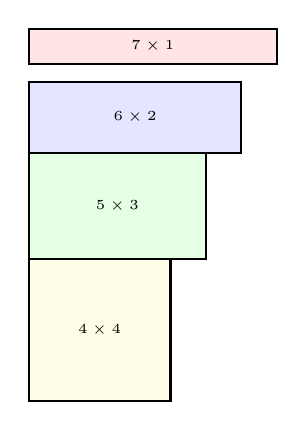
\begin{tikzpicture}[scale=0.45]
  \draw[thick,fill=red!10] (0,0) rectangle (7,1);
  \node at (3.5,0.5) {\tiny $7 \times 1$};
  \draw[thick,fill=blue!10] (0,-2.5) rectangle (6,-0.5);
  \node at (3,-1.5) {\tiny $6 \times 2$};
  \draw[thick,fill=green!10] (0,-5.5) rectangle (5,-2.5);
  \node at (2.5,-4) {\tiny $5 \times 3$};
  \draw[thick,fill=yellow!10] (0,-9.5) rectangle (4,-5.5);
  \node at (2,-7.5) {\tiny $4 \times 4$};
\end{tikzpicture}
\end{center}
\end{questionText}
\choiceA{A given perimeter determines exactly one rectangle}
\choiceB{A given perimeter allows more than one rectangle}
\choiceC{All rectangles with the same perimeter have the same area}
\choiceD{It is impossible for multiple rectangles to share a perimeter}
\correctAnswer{B}
\explanation{The four rectangles all have perimeter $16$ cm ($2(7+1) = 2(6+2) = 2(5+3) = 2(4+4) = 16$) but different shapes. A given perimeter allows many rectangles.}
\end{practiceQuestion}

\begin{practiceQuestion}{6-4-q15}{mc}
\begin{questionText}
You know two angles of a triangle are $55°$ and $65°$ and a non-included side is $9$ cm. This is an example of:
\end{questionText}
\choiceA{SSS}
\choiceB{SAS}
\choiceC{ASA}
\choiceD{AAS}
\correctAnswer{D}
\explanation{Two angles and a non-included side is AAS (Angle-Angle-Side). This produces a unique triangle.}
\end{practiceQuestion}

\begin{practiceQuestion}{6-5-q04}{mc}
\begin{questionText}
You slice a sphere with any flat plane. What shape is the cross-section?
\end{questionText}
\choiceA{Oval}
\choiceB{Rectangle}
\choiceC{Circle}
\choiceD{It depends on the angle of the cut}
\correctAnswer{C}
\explanation{Every cross-section of a sphere is a circle. The size of the circle depends on where you cut, but the shape is always a circle.}
\end{practiceQuestion}

\begin{practiceQuestion}{7-3-q17}{mc}
\begin{questionText}
What is the area of a circle with a radius of $1.5$ meters? Use $\pi \approx 3.14$.
\end{questionText}
\choiceA{$4.71$ m$^2$}
\choiceB{$7.065$ m$^2$}
\choiceC{$9.42$ m$^2$}
\choiceD{$14.13$ m$^2$}
\correctAnswer{B}
\explanation{$A = \pi r^2 = 3.14 \times (1.5)^2 = 3.14 \times 2.25 = 7.065$ m$^2$.}
\end{practiceQuestion}

\begin{practiceQuestion}{7-4-q26}{gmc}
\begin{questionText}
What is the area of the shaded composite figure on the grid? Each square is $1$ cm by $1$ cm.

\begin{center}
\begin{tikzpicture}[scale=0.5]
  \draw[step=1,gray!30,thin] (0,0) grid (10,7);
  \fill[funBlue!20] (1,1) -- (9,1) -- (9,4) -- (6,4) -- (6,6) -- (4,6) -- (4,4) -- (1,4) -- cycle;
  \draw[thick,funBlue] (1,1) -- (9,1) -- (9,4) -- (6,4) -- (6,6) -- (4,6) -- (4,4) -- (1,4) -- cycle;
  \node[below] at (1,1) {\small $(1{,}1)$};
  \node[below] at (9,1) {\small $(9{,}1)$};
  \node[right] at (9,4) {\small $(9{,}4)$};
  \node[right] at (6,4) {\small $(6{,}4)$};
  \node[above] at (6,6) {\small $(6{,}6)$};
  \node[above] at (4,6) {\small $(4{,}6)$};
  \node[left] at (4,4) {\small $(4{,}4)$};
  \node[left] at (1,4) {\small $(1{,}4)$};
\end{tikzpicture}
\end{center}
\end{questionText}
\choiceA{$24$ cm$^2$}
\choiceB{$28$ cm$^2$}
\choiceC{$32$ cm$^2$}
\choiceD{$36$ cm$^2$}
\correctAnswer{B}
\explanation{Bottom rectangle: $8 \times 3 = 24$ cm$^2$. Top rectangle: $2 \times 2 = 4$ cm$^2$. Total: $24 + 4 = 28$ cm$^2$.}
\end{practiceQuestion}

\begin{practiceQuestion}{7-5-q20}{sa}
\begin{questionText}
A cube has a side length of $7$ m. What is its surface area?
\end{questionText}
\correctAnswer{$294$ m$^2$}
\explanation{$SA = 6s^2 = 6 \times 49 = 294$ m$^2$.}
\end{practiceQuestion}

\begin{practiceQuestion}{7-6-q16}{mc}
\begin{questionText}
A rectangular prism has a volume of $240$ cm$^3$. Its base is $8$ cm by $6$ cm. What is the height?
\end{questionText}
\choiceA{$4$ cm}
\choiceB{$5$ cm}
\choiceC{$6$ cm}
\choiceD{$10$ cm}
\correctAnswer{B}
\explanation{$B = 8 \times 6 = 48$ cm$^2$. $h = V \div B = 240 \div 48 = 5$ cm.}
\end{practiceQuestion}

\begin{practiceQuestion}{8-1-q30}{gsa}
\begin{questionText}
The table shows the results of a random sample of $80$ people about their preferred pet.

\begin{center}
\begin{tabular}{|l|c|}
\hline
\textbf{Pet} & \textbf{Number} \\
\hline
Dog & $32$ \\
\hline
Cat & $24$ \\
\hline
Fish & $12$ \\
\hline
Bird & $8$ \\
\hline
Other & $4$ \\
\hline
\end{tabular}
\end{center}

What percent of the sample prefers cats? If the population is $5{,}000$, predict how many prefer cats.
\end{questionText}
\correctAnswer{$30\%$; $1{,}500$ people}
\explanation{$\frac{24}{80} = 0.30 = 30\%$. Then $30\%$ of $5{,}000 = 1{,}500$.}
\end{practiceQuestion}

\begin{practiceQuestion}{8-3-q01}{mc}
\begin{questionText}
Class A has a mean test score of $78$ and Class B has a mean test score of $85$. What can you conclude?
\end{questionText}
\choiceA{Every student in Class B scored higher than every student in Class A}
\choiceB{Class B scored higher on average than Class A}
\choiceC{Class A and Class B have the same scores}
\choiceD{Class A has more students than Class B}
\correctAnswer{B}
\explanation{The mean tells us the average performance. Class B scored higher on average, but individual scores may overlap.}
\end{practiceQuestion}

\begin{practiceQuestion}{8-4-q14}{mc}
\begin{questionText}
Data: $42, 45, 47, 50, 53, 55, 58$. Find $Q_1$ and $Q_3$.
\end{questionText}
\choiceA{$Q_1 = 45$, $Q_3 = 55$}
\choiceB{$Q_1 = 42$, $Q_3 = 58$}
\choiceC{$Q_1 = 47$, $Q_3 = 53$}
\choiceD{$Q_1 = 44$, $Q_3 = 56$}
\correctAnswer{A}
\explanation{Median $= 50$. Lower half: $42, 45, 47$, so $Q_1 = 45$. Upper half: $53, 55, 58$, so $Q_3 = 55$.}
\end{practiceQuestion}

\begin{practiceQuestion}{8-7-q03}{mc}
\begin{questionText}
A double bar graph is used to:
\end{questionText}
\choiceA{Show one data set over time}
\choiceB{Compare two data sets using side-by-side bars}
\choiceC{Show parts of a whole}
\choiceD{Display individual data points}
\correctAnswer{B}
\explanation{Double bar graphs place two sets of bars side by side for each category so you can compare them directly.}
\end{practiceQuestion}

\begin{practiceQuestion}{9-4-q21}{sa}
\begin{questionText}
A bag has $6$ red, $4$ blue, and $10$ white marbles. Write the probability model by listing $P(\text{red})$, $P(\text{blue})$, and $P(\text{white})$ as fractions in simplest form.
\end{questionText}
\correctAnswer{$P(\text{red}) = \frac{3}{10}$, $P(\text{blue}) = \frac{1}{5}$, $P(\text{white}) = \frac{1}{2}$}
\explanation{Total: $20$. $P(\text{red}) = \frac{6}{20} = \frac{3}{10}$, $P(\text{blue}) = \frac{4}{20} = \frac{1}{5}$, $P(\text{white}) = \frac{10}{20} = \frac{1}{2}$.}
\end{practiceQuestion}

\begin{practiceQuestion}{9-6-q26}{gmc}
\begin{questionText}
The table shows all possible sums when two dice are rolled. What is the probability of rolling a sum of $8$?

\begin{center}
\begin{tabular}{|c|c|c|c|c|c|c|}
\hline
$+$ & \textbf{1} & \textbf{2} & \textbf{3} & \textbf{4} & \textbf{5} & \textbf{6} \\
\hline
\textbf{1} & $2$ & $3$ & $4$ & $5$ & $6$ & $7$ \\
\hline
\textbf{2} & $3$ & $4$ & $5$ & $6$ & $7$ & \cellcolor{funBlue!20}$8$ \\
\hline
\textbf{3} & $4$ & $5$ & $6$ & $7$ & \cellcolor{funBlue!20}$8$ & $9$ \\
\hline
\textbf{4} & $5$ & $6$ & $7$ & \cellcolor{funBlue!20}$8$ & $9$ & $10$ \\
\hline
\textbf{5} & $6$ & $7$ & \cellcolor{funBlue!20}$8$ & $9$ & $10$ & $11$ \\
\hline
\textbf{6} & $7$ & \cellcolor{funBlue!20}$8$ & $9$ & $10$ & $11$ & $12$ \\
\hline
\end{tabular}
\end{center}
\end{questionText}
\choiceA{$\frac{4}{36}$}
\choiceB{$\frac{5}{36}$}
\choiceC{$\frac{6}{36}$}
\choiceD{$\frac{8}{36}$}
\correctAnswer{B}
\explanation{Outcomes with sum $8$: $(2,6), (3,5), (4,4), (5,3), (6,2)$ — that is $5$. $P = \frac{5}{36}$.}
\end{practiceQuestion}

\begin{practiceQuestion}{9-7-q18}{mc}
\begin{questionText}
In a simulation of $100$ free throws, a basketball player makes $78$. If the player's actual success rate is $75\%$, is the simulation result reasonable?
\end{questionText}
\choiceA{No, any difference means the simulation is wrong}
\choiceB{Yes, $78\%$ is close to $75\%$, which is expected variation}
\choiceC{No, because $78$ is not equal to $75$}
\choiceD{Yes, but only if exactly $75$ are made}
\correctAnswer{B}
\explanation{$\frac{78}{100} = 0.78$ vs. theoretical $0.75$. A small difference in $100$ trials is normal and expected.}
\end{practiceQuestion}
